% [原文 p.77]
对 $S^3$ 中带有 framing 的链环 $L$、$L'$，沿其作 Dehn 手术，得到三维流形 $M_L$、$M_{L'}$。众所周知，二者同胚的条件是：$L'$ 可由 $L$ 经有限次称为 Kirby 操作（Kirby move）的局部变形得到。这里，我们采用 Fenn--Rourke（[26]）给出的表述形式，把它作为定理陈述出来。

\begin{theorem}{2.13}（Kirby 操作）\quad 三维流形 $M_L$、$M_{L'}$ 同胚，当且仅当 $L'$ 可由 $L$ 经图2.19 所示的链环局部变形的有限次重复得到。其中，$n$ 表示穿过带有 framing $\varepsilon$（$\varepsilon=\pm 1$）的平凡纽结的股数。特别地，$n=0$ 的情形表示如下操作及其逆操作：从三维球体中挖去一个带有 framing $\varepsilon$ 的平凡纽结。
\end{theorem}

\begin{figure}[htbp]
  \centering
  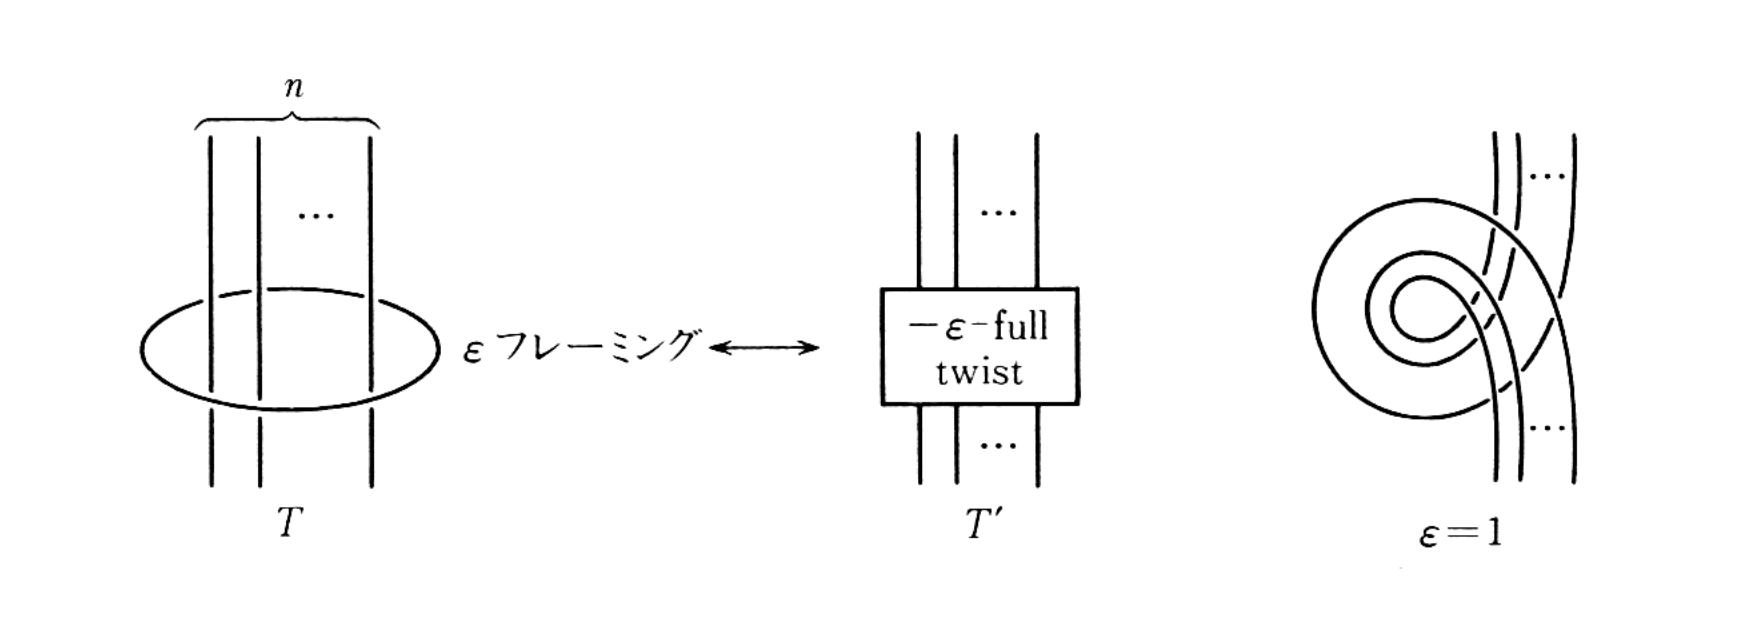
\includegraphics[width=0.78\textwidth]{figures/fig2.19.png}
  \figtitle{2.19}{Kirby 操作。右图为 $\varepsilon=1$ 时的 tangle $T'$。（原书 p.77）}
\end{figure}

设 $L$ 是 $S^3$ 中带有 framing 的链环，其成分为 $L_1,\dots,L_m$。对互不相同的 $i,j$，以 $L_i\cdot L_j$ 表示 $L_i$ 与 $L_j$ 的环绕数；又令 $L_i\cdot L_i$ 为确定 $L_i$ 的 framing 的整数。以 $L_i\cdot L_j$ 为 $(i,j)$ 元作 $m$ 阶方阵 $A$，称 $A$ 为 $L$ 的环绕矩阵（linking matrix）。$A$ 是对称矩阵。把 $A$ 的正特征值个数记作 $n_+$，负特征值个数记作 $n_-$。链环 $L$ 的环绕矩阵的符号差 $\sigma(L)$ 定义为 $n_+-n_-$。它等于四维流形 $W_L$ 的相交形式的符号差。

% [Tutor Note: 对 $i\ne j$，$L_i\cdot L_j$ 是两条不同分支的环绕数；对角元 $L_i\cdot L_i$ 则是确定 $L_i$ 的 framing 的整数，须理解为 $L_i$ 与其平行副本的配对，并不是 $L_i$ 与自身的环绕数。]

为定义三维流形的 Witten 不变量，先按第 1 章的内容准备一些记号。Lie 代数 $\fg$ 取为 $\fsl_2(\C)$。固定正整数 $k$，把仿射 Lie 代数 $\hat{\fg}$ 的 level $k$ 的最高权集合记作 $P_+(k)$。
% [原文 p.78]
具体地，
\[
  P_+(k)=\{0,1,\dots,k\}
\]
如 §1.2 所述，对每个 $\lambda\in P_+(k)$，都有 $\hat{\fg}$ 的最高权为 $\lambda$ 的不可约表示 $\cH_\lambda$ 与之对应。Virasoro 代数通过 Sugawara 形式作用在 $\cH_\lambda$ 上，其中心的值（中心荷）为
\[
  c=\frac{3k}{k+2}.
\]
这里令
\[
  C=\exp\Bigl(2\pi\sqrt{-1}\,\frac{c}{24}\Bigr)^{-3}.
\]
% [Tutor Note: 原书此处的指数是 $-3$，不是 $-1$：$C=\exp(2\pi\sqrt{-1}c/24)^{-3}$。后文定理 2.16 中的 $C^{\sigma(L)}$ 用的就是这个量，转抄时不要漏掉指数。]

如 §1.6 所述，$A_1^{(1)}$ 型仿射 Lie 代数 level $k$ 的特征标 $\chi_\lambda$（$\lambda\in P_+(k)$）在 $SL_2(\Z)$ 的作用下按
\[
  \chi_\lambda\Bigl(-\frac{1}{\tau}\Bigr)=\sum_{\mu}S_{\lambda\mu}\chi_\mu(\tau),
\]
\[
  \chi_\lambda(\tau+1)=\exp\Bigl(2\pi\sqrt{-1}\bigl(\Delta_\lambda-\frac{c}{24}\bigr)\Bigr)\chi_\lambda(\tau)
\]
变换。这里 $\tau$ 是复上半平面的元素；如 (1.42)、(1.43) 所记，$S_{\lambda\mu}$、$\Delta_\lambda$ 具体为
\[
  S_{\lambda\mu}=\sqrt{\frac{2}{k+2}}\,\sin\frac{(\lambda+1)(\mu+1)\pi}{k+2},
\]
\[
  \Delta_\lambda=\frac{\lambda(\lambda+2)}{4(k+2)}.
\]
这些量在下面构造三维流形不变量的描述中起基本作用。由
\[
  S(\tau)=-\frac{1}{\tau},\qquad T(\tau)=\tau+1
\]
确定的分式线性变换 $S$、$T$
% [原文 p.79]
满足
\[
  S^2=(ST)^3=I.
\]
利用这一点，可得下述引理。

\begin{lemma}{2.14}
  上面的 $S_{\lambda\mu}$ 满足如下关系式：
  \[
    C\sum_{\mu}S_{\lambda\mu}S_{\mu\nu}\exp\bigl(2\pi\sqrt{-1}(\Delta_\lambda+\Delta_\mu+\Delta_\nu)\bigr)=S_{\lambda\nu}.
  \]
\end{lemma}

% [Tutor Note: 引理 2.14 中 $\lambda$、$\nu$ 是固定的外指标，求和只对中间的 $\mu$ 进行；指数里三个 $\Delta$ 的下标分别为 $\lambda,\mu,\nu$，不要漏掉 $\Delta_\mu$。]

设 $L$ 是 $S^3$ 中带有定向与 framing 的链环，其成分为 $L_1,\dots,L_m$。对每个成分，用 $\lambda:\{1,\dots,m\}\to P_+(k)$ 赋予 level $k$ 的最高权，前一节由此定义了不变量 $J(L;\lambda(1),\dots,\lambda(m))$。关于这个不变量，下述结论成立。

\begin{proposition*}{2.15}
  对图2.20 所示 Hopf 链环 $H$ 的两个成分赋予 level $k$ 的最高权 $\lambda$、$\mu$，则有
  \[
    J(H;\lambda,\mu)=\frac{S_{\lambda\mu}}{S_{00}}.
  \]
\end{proposition*}

\begin{proof}
  把 Hopf 链环按图2.20 表示。由前一节引理 2.8 给出的关于 cabling 的结果，可得
  \[
    \exp\bigl(2\pi\sqrt{-1}(-\Delta_\lambda-\Delta_\mu)\bigr)J(H;\lambda,\mu)
    =\sum_{\nu}N_{\lambda\mu}^{\ \ \nu}\exp\bigl(2\pi\sqrt{-1}(-\Delta_\nu)\bigr)\frac{S_{0\nu}}{S_{00}}.
  \]
  应用命题 1.22 所述的 Verlinde 等式与引理 2.14，即得欲证的结论。
\end{proof}

\begin{figure}[htbp]
  \centering
  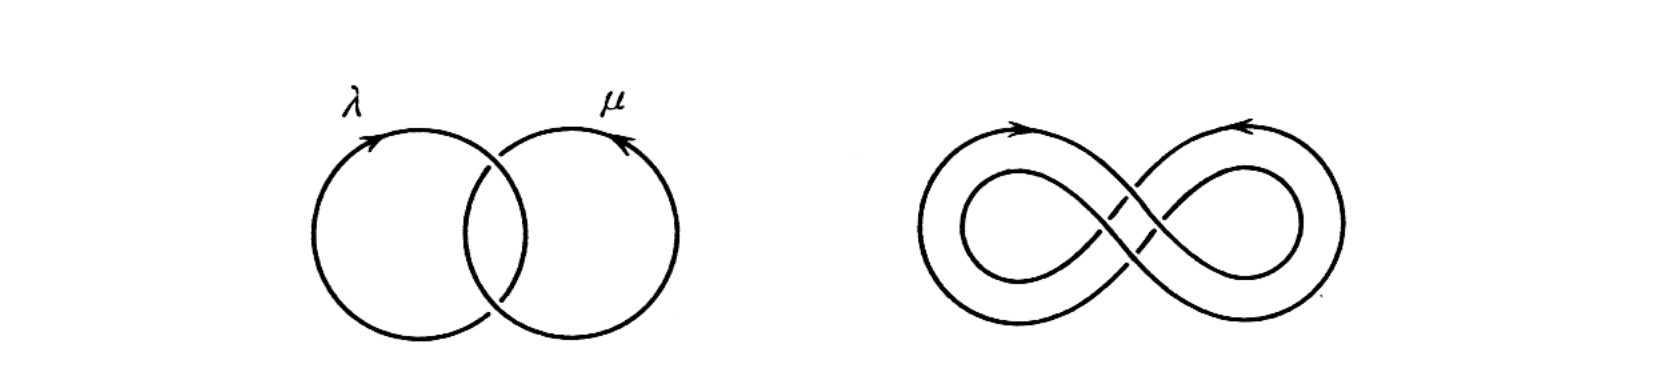
\includegraphics[width=0.62\textwidth]{figures/fig2.20.png}
  \figtitle{2.20}{Hopf 链环（原书 p.79）}
\end{figure}

下面的定理是本节的中心结果。

\begin{theorem}{2.16}
  设 $M$ 是紧致、无边界、带有定向的三维流形。若 $M$ 可由三维球面 $S^3$ 中带有 framing 的链环 $L$
% [原文 p.80]
  沿其作 Dehn 手术得到，则
  \[
    \resizebox{0.98\textwidth}{!}{$\displaystyle
      Z_k(M)=S_{00}\,C^{\sigma(L)}\sum_{\lambda}S_{0,\lambda(1)}\cdots S_{0,\lambda(m)}J(L;\lambda(1),\dots,\lambda(m))$}
  \]
  是 $M$ 的拓扑不变量。其中，链环 $L$ 由 $m$ 个成分 $L_j$（$1\le j\le m$）组成，$\lambda$ 遍历给链环各成分赋 level $k$ 权的所有映射 $\lambda:\{1,\dots,m\}\to P_+(k)$。
\end{theorem}

定理所说的拓扑不变性，其确切含义如下。把沿链环 $L$ 作 Dehn 手术所得的三维流形记作 $M_L$。定理中公式的右端依赖于链环 $L$，故将它记作 $Z_k(M_L)$。此时，对两个链环 $L$、$L'$，若存在保向同胚 $M_L\cong M_{L'}$，则 $Z_k(M_L)=Z_k(M_{L'})$ 成立。另外请注意：定理中为定义 $J(L;\lambda(1),\dots,\lambda(m))$，需要指定链环 $L$ 的定向；但像 $Z_k(M)$ 的右端那样对 $\lambda$ 求和之后，所得结果与链环 $L$ 的定向无关。

\begin{proof}
  下面证明 $Z_k(M_L)$ 在 Kirby 操作下不变。先考虑图2.19 中 $n=0$ 的情形。在引理 2.14 中取 $\lambda=\nu=0$，得
  \[
    C\sum_{\mu\in P_+(k)}S_{0\mu}\frac{S_{0\mu}}{S_{00}}\exp\bigl(2\pi\sqrt{-1}\,\Delta_\mu\bigr)=1.
  \]
  对链环不变量 $J$，用平凡纽结情形下的取值（引理 2.9）以及关于 framing 的命题 2.6，即得 Kirby 操作在 $n=0$ 情形下 $Z_k(M_L)$ 的不变性。

  其次处理 $n=1$ 的情形。利用命题 2.12 所述的链环不变量 $J$ 的分解法则，只需对图2.20 所示 Hopf 链环的情形验证即可。此时，利用命题 2.15 关于 Hopf 链环的结果，以及在引理 2.14 中取 $\nu=0$ 所得的式子
  \[
    C\sum_{\mu\in P_+(k)}S_{0\mu}\frac{S_{\lambda\mu}}{S_{00}}\exp\bigl(2\pi\sqrt{-1}\,\Delta_\mu\bigr)
    =\exp\bigl(-2\pi\sqrt{-1}\,\Delta_\lambda\bigr)\frac{S_{0\lambda}}{S_{00}},
  \]
  即可得到结论。

  以下对 $n$ 作归纳法证明。局部地看，图2.19 的 $(n,n)$ tangle
% [原文 p.81]
  $T$、$T'$ 的各成分如图2.21 左那样赋予权，则只需证明对应的 tangle 算子满足
  \[
    C^{\sigma(L)}\sum_{\mu}S_{0\mu}J(T;\mu,\lambda_1,\dots,\lambda_n)
    =C^{\sigma(L')}J(T';\lambda_1,\dots,\lambda_n).
  \]
  这里，$T'$ 表示对 $T$ 施以上述 Kirby 操作所得的链环的一部分。按前一节引理 2.8 说明的方法，把 $n$ 条中的前 2 条归并到一起（如图2.21 所示），即可把欲证等式的左端写成关于 $(n-1,n-1)$ tangle $T''$ 的 tangle 算子
  \[
    J(T'';\mu,\nu,\lambda_3,\dots,\lambda_n).
  \]
  对其中每一项用归纳法假设，再考察 $\sigma(L)$ 在 Kirby 操作下的变化，即得欲证的结论。
\end{proof}

% [Tutor Note: 证明中 $\sigma(L)$ 与 $\sigma(L')$ 之差不是零，而是被 $C^{\sigma(L)}$、$C^{\sigma(L')}$ 两个因子吸收；如果误以为 Kirby 操作保持符号差，就会看不出这一步为何成立。]

\begin{figure}[htbp]
  \centering
  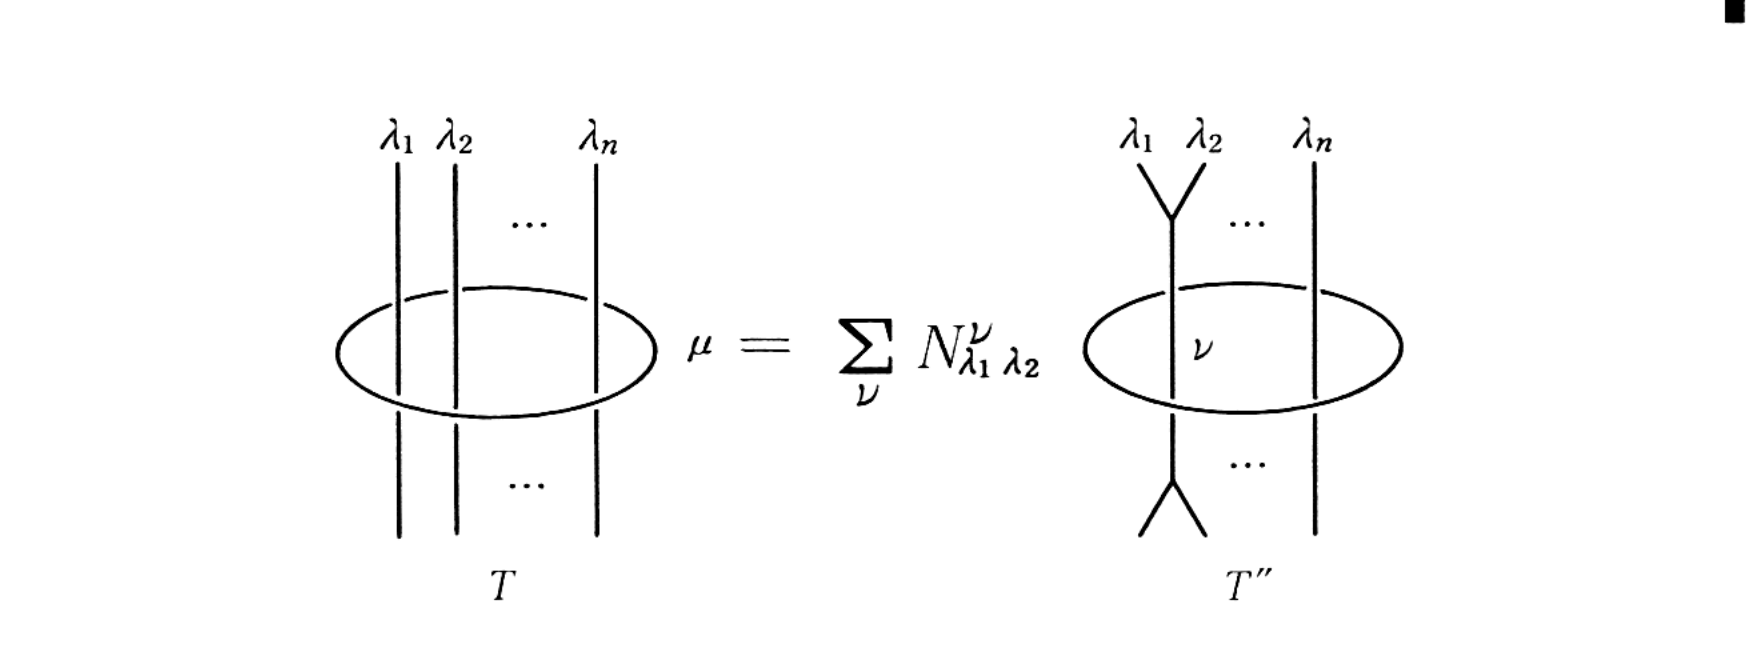
\includegraphics[width=0.78\textwidth]{figures/fig2.21.png}
  \figtitle{2.21}{原书无图注（原书 p.81）}
\end{figure}

这样得到的三维流形的拓扑不变量 $Z_k(M)$，称为附属于 Lie 代数 $\fsl_2(\C)$、level 为 $k$ 的\textbf{Witten 不变量}。下面举几个 Witten 不变量的简单计算例子。对三维球面 $S^3$，由定义立即看出
\[
  Z_k(S^3)=S_{00}.
\]
又对直积 $S^1\times S^2$，由于 $S^1\times S^2$ 可由 $S^3$ 中framing 为 $0$ 的平凡纽结沿其作 Dehn 手术得到，故算得
\[
  Z_k(S^1\times S^2)=1.
\]
% [Tutor Note: 这两个例子给出的是归一化基准：$S^3$ 的值取 $S_{00}$ 而非 $1$，$S^1\times S^2$ 的值恰好为 $1$。后文命题 2.17 中的因子 $1/S_{00}$ 正是为了抵消 $S^3$ 这一归一化。]

% [原文 p.82]
下面列举 Witten 不变量的几条基本性质。

\begin{proposition*}{2.17}
  对三维流形的连通和，有
  \[
    Z_k(M_1\# M_2)=\frac{1}{S_{00}}Z_k(M_1)Z_k(M_2).
  \]
\end{proposition*}

\begin{proof}
  设 $M_1$、$M_2$ 分别由沿链环 $L_1$、$L_2$ 的 Dehn 手术给出。此时连通和 $M_1\# M_2$ 可由沿链环 $L$ 的 Dehn 手术得到，而 $L$ 是分别含于互不相交的两个三维球体 $B_1$、$B_2$ 中的链环 $L_1$、$L_2$ 之并。因此，结合关于链环不变量的命题 2.10，即得结论。
\end{proof}

\begin{proposition*}{2.18}
  把 $M$ 的定向反转所得流形记作 $-M$，则
  \[
    Z_k(-M)=\overline{Z_k(M)}.
  \]
\end{proposition*}

\begin{proof}
  设 $M$ 由沿链环 $L$ 的 Dehn 手术给出。此时 $-M$ 由沿 $L$ 的镜像的 Dehn 手术得到，故由命题 2.11 立即得证。
\end{proof}

% [Tutor Note: 命题 2.18 中右端的横线是复共轭，不是闭包也不是取逆；它与命题 2.11（镜像与复共轭的对应）是同一事实的两种说法。]

这里，我们以共形场理论为基础构造了 Witten 不变量 $Z_k(M)$；而在 Reshetikhin--Turaev（[43]）中，用的是量子群参数取 1 的单位根时的表示论，给出了 Witten 不变量的 Dehn 手术描述。

把上述构造推广到三维流形含链环的情形，也是可行的。设 $L$ 是三维流形 $M$ 内带有定向与 framing 的链环，其成分为 $L_1,\dots,L_n$，并对它们赋 level $k$ 的最高权 $\lambda_1,\dots,\lambda_n$。设 $(M,L)$ 由 $(S^3,L')$ 中带有 framing 的链环 $N=N_1\cup\cdots\cup N_m$ 沿其作 Dehn 手术得到。这里，链环 $N$ 取成与 $L'$ 不相交。此时 $(M,L)$ 的不变量 $Z_k(M,L;\lambda_1,\dots,\lambda_n)$ 由
\[
  \resizebox{0.98\textwidth}{!}{$\displaystyle
    S_{00}\,C^{\sigma(N)}\sum_{\mu}S_{0,\mu(1)}\cdots S_{0,\mu(m)}J(L'\cup N;\lambda_1,\dots,\lambda_n,\mu(1),\dots,\mu(m))$}
\]
确定。

% CHUNK ch02c DONE
